
\documentclass[runningheads]{llncs}
\usepackage{graphicx}
\usepackage{amsfonts}
\usepackage{mathtools}
\usepackage{tikz}
\usetikzlibrary{shapes.geometric, arrows}

\tikzstyle{startstop} = [rectangle, rounded corners, minimum width=3cm, minimum height=1cm,text centered, draw=black, fill=red!30]
\tikzstyle{process} = [rectangle, minimum width=2cm, minimum height=1cm, text centered, text width=4cm, draw=black, fill=orange!30]
\tikzstyle{decision} = [diamond, minimum width=3cm, minimum height=1cm, text centered, draw=black, fill=green!30]
\tikzstyle{arrow} = [thick,->,>=stealth]

\begin{document}

\title{Modeling Personality Traits-based Friendship Networks among Agents}

\author{Reuben Bernard Francis (45539979)}
\institute{Macquarie University}
%
\maketitle              % typeset the header of the contribution

%
%
%
\section{Introduction}
Psychology and network analysis are terms that have been used together before. Psychologists have established non-trivial associations between personality and social network structures with network theory. This study however, backed up empirically still overlook theoretical analysis. The models created for these relationships suffer the same. We create a generative model for personality-based friendship networks, exploring traits like extraversion and agreeableness. A social network has never been emphatically mentioned in-hand with personality and friendship formation. The two traits mentioned happen to empirically resonate positively with degree. We explain how personality changes can reflect an effect of personality on the friendship network structure.

The spread of network theory in psychology has sparked the relationship between personality and network structure \cite{ref_2}. This empirical grounding is based on previous correlational studies, a practice of utilizing statistical tools on social networks to realize relations like how extraversion and agreeableness relate consistently to personal networks, and openness predicts network diversity. This gets harder to be explained theoretically. Our motivating scenarios is to theorize that personality changes on friendships can amount to the effect of personality on network structure. Previously mentioned, extraversion and agreeableness hold empirically strong and therefore validate our proposed model. 

\section{Related Work}
Examining the empirical study based on personality and friendship networks, we review how they aren’t sufficient to support our proposal, explaining how existing models aren’t enough.  Representative explanations of personality and social networks is our focus.\cite{ref_2} took the effort of reviewing 30 articles, understood that openness has strong associations in personal networks while extraversion and agreeableness were relatable within personal networks rather than workplaces. A study by \cite{ref_3} stated that self-monitoring helps predict in-degree centrality in expressive and instrumental networks after analyzing 138 independent data samples.

Research like \cite{ref_4} helped understand friendship networks, a simple observation within a few students explaining how extraverts have more friends than introverts. This study was extended by \cite{ref_5}, who sampled sociometric nominations and self-ratings on personality traits, inferring extraversion gathered higher out-degree while individuals high on agreeableness had higher in-degree. A few other studies by \cite{ref_6,ref_7,ref_8,ref_9,ref_10} help conclude how extraversion and agreeableness are correlated with degree in friendship network structures. We now emphasis personality and friendship network models, a number of them like \cite{ref_12}’s game-theory based understanding of racial segregation in friendship networks answer questions of complex friendship patterns but doesn’t implement an individual’s personality. A generative model for social network by \cite{ref_13} had personality in the equation but concerned with animal social behavior in terms of boldness.

We now study the science of personality and friendship, \cite{ref_17} explains how personality is a set of psychological traits that help enduring distinctive patterns of feelings, thoughts, and behaviors of an individual. A commonly known model, the Five Factor Model (FFM) uses five orthogonal dimensions predicting mentioned patterns. The Five Factors (Big Five) traits are Openness, Conscientiousness, Extraversion, Agreeableness, Neuroticism. \cite{ref_20} defines friends being more than just casual meetings of strangers. This ideology was extended by \cite{ref_21}, noticing how friendships are dynamic, they roughly follow a course of formation, maintenance, and possibly dissolution.

\section{Identified Methodology}
We deal with the interdependence of personality and friendship, noticing extraversion and agreeableness as positive traits for friendships development \cite{ref_16}. Former requires low acquaintance to become more comfortable, being able to find strangers likable \cite{ref_22}, while the latter shows how agreeable people are likable, one person in a relationship having this trait are likely to feel comfortable. We therefore propose a generative model for friendship networks with personality, following rules mentioned in our study of personality and friendship, understanding how each agent’s friendship dissolution depends on personality. This model is basically an extension of heterogenous network models \cite{ref_24}.

\subsection{Model Formation}
We start with an initial network that eventually generates an order of undirected simple networks, in each sequence however, the model follows three subroutines: adding new node ($\alpha$) and forming edges from them, forming edges between existing nodes ($\beta$), and dissolving edges between existing nodes ($\gamma$). Figure \ref{fig_1} shows an advanced description of the proposed model.

An agents’ personality and degree formulate probability distributions for each formulating or dissolving edge. Following elements help define our model.
\begin{enumerate}
  \item $\mathcal{P}$ is an arbitrary space. Agents’ personality referred by $p$
  \item $p$ is a real, non-negative function having unit measure over $\mathcal{P}$, which is the probability distribution of population personality.
  \item $c_\alpha,c_\beta,$ and $c_\gamma$ indicates the probability that subroutine $\alpha, \beta$, and $\gamma$ occur at each round
  \item $\pi_\alpha,\pi_\beta,$ and $\pi_\gamma$ functions are used to describe how an individual’s personality affect their difference in friendship formation and maintenance.
  \item $m_\alpha,m_\beta,$ and $m_\gamma$ functions are same as previous but show agents’ difference in friendship development. 
\end{enumerate}

\begin{figure}
\centering
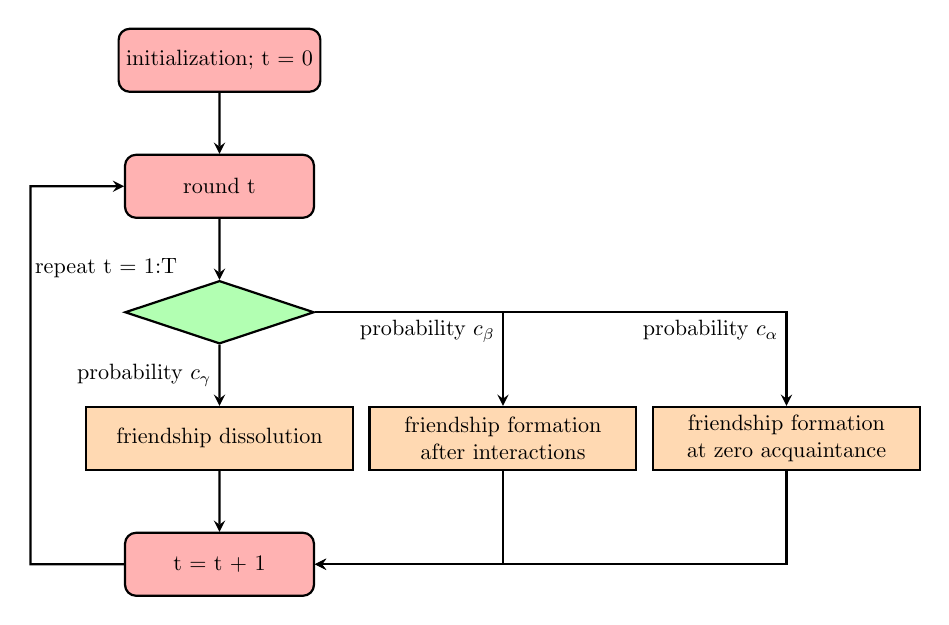
\begin{tikzpicture}[node distance=2cm,thick,scale=0.8, every node/.style={transform shape}]
\node (init) [startstop] {initialization; t = 0};
\node (round) [startstop,below of=init] {round t};
\node (dec) [decision, below of=round] {};
\node (pro1) [process, below of=dec] {friendship dissolution};
\node (pro2) [process, right of=pro1, xshift=2.5cm] {friendship formation after interactions};
\node (pro3) [process, right of=pro2, xshift=2.5cm] {friendship formation at zero acquaintance};
\node (stop) [startstop,below of=pro1] {t = t + 1};
\draw [arrow] (init) -- (round);
\draw [arrow] (round) -- (dec);
\draw [arrow] (dec) -- node[anchor=east] {probability $c_\gamma$} (pro1);
\draw [arrow] (dec) -| node[anchor=north east] {probability $c_\beta$} (pro2);
\draw [arrow] (dec) -| node[anchor=north east] {probability $c_\alpha$} (pro3);
\draw [arrow] (pro1) -- (stop);
\draw [arrow] (pro2) |- (stop);
\draw [arrow] (pro3) |- (stop);
\draw [arrow] (stop) -- (-3,-8) |- node[xshift=1.2cm,yshift=-1.3cm] {repeat t = 1:T} (round);

\end{tikzpicture}
\caption{Flowchart representing proposed model description} \label{fig_1}
\end{figure}

Our generated undirected simple graph $G^{(t)}=\left(V^{(t)}, E^{(t)}\right)$ at round t has each node $v_{i} \in V^{(t)}$ associated with personality $p_{i} \in P$ assumed fixed during model evolution. Sometimes overloading $v_{i}^{(t)}$ is denoted as $\left(p_{i}, k_{i}(t)\right)$, where $k_{i}(t)$ is degree of $v_{i}$ at end of round $t$. Here are the rules for network evolution.

\begin{enumerate}
    \item 	Start initial process (round 0) with $N_0$ agents, $L_0$ links and arbitrary personality $p_i \in \mathcal{P}$
    \item   At each round $t$, model enters one of three subroutines with probability $\left(c_{\alpha}, c_{\beta}, c_{\gamma}\right)$:
    \begin{enumerate}
        \item 	{\itshape Subroutine $\alpha$: adding agent and friendship formation at zero acquaintance:} 
        Enters with probability $c_\alpha$, agent $v_x$ with $m_\alpha(p_x)$ links is added to the network, this agent is randomly assigned a personality $p_x$ according to distribution p. 
        
        For each $m_\alpha (p_x)$ iterations, node $v_{i}$ in $V^{(t-1)}$ is selected with probability proportional to $\pi_{\alpha}\left(v_{i}^{(t-1)}, v_{x}^{(t-1)}\right)$, and edge $\left(v_{x}, v_{i}\right)$ is formed. In conclusion, when newcomers enter a society, they form friendship with zero acquaintance.
        
        \item  {\itshape Subroutine $\beta$: friendship formation after interactions:} Enters with probability $c_{\beta},$ existing node $v_{x} \in V^{(t-1)}$ is selected uniformly at random. 
        
        For each $m_{\beta}\left(p_{x}\right)$ iterations, node $v_{i}$ in $V^{(t-1)}-N^{(t-1)}\left(v_{x}\right)=\overline{N^{(t-1)}\left(v_{x}\right)}$ is selected with probability proportional to $\pi_{\beta}\left(v_{i}^{(t-1)}, v_{x}^{(t-1)}\right),$ and edge $\left(v_{x}, v_{i}\right)$ is formed. In conclusion, agents already existing in society may still make friends with acquainted others.
        
        \item  {\itshape Subroutine $\gamma$: friendship dissolution:} Enters with probability $c_{\gamma},$ existing node $v_{x} \in V^{(t-1)}$ is selected uniformly at random. 
        
        For each $m_{\gamma}\left(p_{x}\right)$ iterations, node $v_{i}$ in $N^{(t-1)}\left(v_{x}\right)$ and neighborhood of $v_{x}$ is selected with probability proportional to $\pi_{\gamma}\left(v_{i}^{(t-1)}, v_{x}^{(t-1)}\right),$ and edge $\left(v_{x}, v_{i}\right)$ is removed. In conclusion, after friendships formed, they might dissolve without maintenance.

    \end{enumerate}
\end{enumerate}

The first two subroutines help friendship formation in two different scenarios, this helps distinguish characterization of likability at zero acquaintance and after interactions \cite{ref_25}. The last subroutine models dissolution without maintenance, this helps distinguish conflict management. For ease of analysis, we can convert our undirected simple graph model to undirected weighted graph. This model replaces $E^{(t)}$ with matrix $W^{(t)}$ initialized to $0,$ then records edge weights between arbitrary nodes after round $t .$ Degree is basically the sum of associating weights, while edge addition and removal are increments and decrements. $V^{(t-1)}$ replaces both $\overline{N^{(t-1)}\left(v_{x}\right)}$ and $N^{(t-1)}\left(v_{x}\right)$ following similar procedures as discussed.

\subsection{Model Analysis}
We try understanding the behavior of our model, we use mean-field approximation, therefore the equation is as follows:
\begin{equation}\label{eq_1}
N_{k}(p, t+1) = N_{k}(p, t)+\delta_{k, m_{\alpha}(p)} c_{\alpha} \rho(p)+c_{\alpha} \Delta_{\alpha}+c_{\beta} \Delta_{\beta}+c_{\gamma} \Delta_{\gamma}
\end{equation}
Where $N_{k}(p, t)$ denotes expected density of node with degree $k$ and probability $p$ right after round $t, \Delta_{\alpha}, \Delta_{\beta},$ and $\Delta_{\gamma}$ denote expected effects from three subroutines; $\delta_{k, m_{\alpha}(p)}$ is a Kronecker delta function. We have two specific cases showing how to analyze the model.

\subsubsection{Edge changes from newcomers being independent of degree:}
Here, $c_{\beta}=c_{\gamma}=0$ since there's only friendship formation. We assume that $\pi_{\alpha}$ is degree independent replaced by $\sigma_{\alpha}$

We have,
\begin{equation}\label{eq_2}
\begin{aligned}
\Delta_{\alpha} &=\frac{N_{k-1}(p, t)-N_{k}(p, t)}{c_{\alpha} t} \sum_{q \in \mathcal{P}} \frac{\sigma_{\alpha}(p, q) \rho(q) m_{\alpha}(q)}{\sum_{r \in \mathcal{P}} \sigma_{\alpha}(r, q) \rho(r)}
\end{aligned}\end{equation}
where,
\begin{equation}\label{eq_3}
A(p)=\sum_{q \in \mathcal{P}} \frac{\sigma_{\alpha}(p, q) \rho(q) m_{\alpha}(q)}{\sum_{r \in \mathcal{P}} \sigma_{\alpha}(r, q) \rho(r)}\end{equation}
Therefore, Eq.\ref{eq_1} can be written as,
$$\begin{aligned}
N_{k}(p, t+1)=& N_{k}(p, t)+\delta_{k, m_{\alpha}(p)} c_{\alpha} \rho(p) +\left(\frac{N_{k-1}(p,t)-N_{k}(p, t)}{t}\right) A(p)
\end{aligned}$$
Which with furter reductions can be written as
\begin{equation}\label{eq_4}
n_{k}(p)=\frac{\rho(p)}{1+A(p)}\left(\frac{A(p)}{1+A(p)}\right)^{k-m_{\alpha}(p)}\end{equation}
We can write expected degree conditioned on personality, 
\begin{equation}\label{eq_5}
\mathbf{E}[k | p]=A(p)+m_{\alpha}(p)\end{equation}

\subsubsection{Edge changes from three subroutines independent of degree:}

Like the previous case, we assume $\pi_{\alpha}, \pi_{\beta}$ and $\pi_{\gamma}$ are all independent of degree replaced by $\sigma_{\alpha}, \sigma_{\beta}$ and $\sigma_{\gamma}$ with domain $P^{2}$

Considering weighted graph model,
\begin{equation}\label{eq_6}
\Delta_{\beta}=\frac{N_{k-1}(p, t)-N_{k}(p, t)}{c_{\alpha} t} B(p)\end{equation}
\begin{equation}\label{eq_7}
\Delta_{\gamma}=\frac{N_{k}(p, t)-N_{k-1}(p, t)}{c_{\alpha} t}(-\Gamma(p))\end{equation}
Where, 
\begin{equation}\label{eq_8}
B(p)=\sum_{q \in \mathcal{P}} \frac{\sigma_{\beta}(p, q) \rho(q) m_{\beta}(q)}{\sum_{r \in \mathcal{P}} \sigma_{\beta}(r, q) \rho(r)}+m_{\beta}(p)\end{equation}
\begin{equation}\label{eq_9}
\Gamma(p)=\sum_{q \in \mathcal{P}} \frac{\sigma_{\gamma}(p, q) \rho(q) m_{\gamma}(q)}{\sum_{r \in \mathcal{P}} \sigma_{\gamma}(r, q) \rho(r)}+m_{\gamma}(p)\end{equation}
Therefore Eq.\ref{eq_1} can be written as, 
\begin{equation}\label{eq_10}
\begin{aligned}
&-\delta_{k, m_{\alpha}(p)} \rho(p) =\left(A(p)+\frac{c_{\beta}}{c_{\alpha}} B(p)\right) n_{k-1}(p)+\frac{c_{\gamma}}{c_{\alpha}} \Gamma(p) n_{k+1}(p) \\
&+\left(-A(p)-\frac{c_{\beta}}{c_{\alpha}} B(p)-\frac{c_{\gamma}}{c_{\alpha}} \Gamma(p)-1\right) n_{k}(p)
\end{aligned}\end{equation}
We skip closed form solution since it’s easier to solve with numeric values at this stage.

\subsection{Effect of Personality on Model}
We use a practical approach to show the effect of personality on friendship network structures. The components of the modeling are specified in Table \ref{tab:table_1}, consistent with \cite{ref_16}’s result summary.

\begin{table}
\begin{center}
\scalebox{0.9}{
\begin{tabular}{ll c c} 
\multicolumn{2}{c}{MODELING SPECIFICATION} \\[1ex]
\hline
Personality Space and Distribution\\
$\mathcal{P}=[-1,1]$\\
$\rho(p)=\frac{1}{2}, \forall p \in \mathcal{P}$\\ [1ex]
\hline
Modeling the Effects of Extraversion\\
$\pi_{\alpha}((p, k),(q, l))=c_{0} p+c_{1}$ & $c_{0}>0, c_{1} \geq c_{0}$\\
$\pi_{\beta}((p, k),(q, l))=c_{2}$ &  $c_{2} \geq 0$\\
$\pi_{\gamma}((p, k),(q, l))=c_{3}$ &  $c_{3} \geq 0$\\
$m_{\alpha}(p)=c_{4}$ &  $c_{4} > 0$\\
$m_{\beta}(p)=c_{5} p+c_{6}$ &  $c_{5}>0, c_{6} \geq c_{5}$\\
$m_{\gamma}(p)=c_{7}$ & $c_{7} \geq 0$\\ [1ex]
\hline
Modeling the Effects of Agreeableness\\
$\pi_{\alpha}((p, k),(q, l))=c_{0}$ & $c_{0} \geq 0$\\
$\pi_{\beta}((p, k),(q, l))=c_{1} p+c_{2}$ & $c_{1}>0, c_{2} \geq c_{1}$\\
$\pi_{\gamma}((p, k),(q, l))=c_{3} p+c_{4}$ & $c_{3}<0, c_{4}\geq-c_{3}$\\
$m_{\alpha}(p)=c_{5}$ & $c_{5}>0$\\
$m_{\beta}(p)=c_{6}$ & $c_{6}>0$\\
$m_{\gamma}(p)=c_{7} p+c_{8}$ & $c_{7}<0,c_{8}\geq-c7$\\ [1ex]
\hline
\end{tabular}}
\caption{\label{tab:table_1}Model Components}
\end{center}
\end{table}


\subsubsection{Modeling the Effects of Extraversion}
The result summary mentioned stated how extraverts are attractive at zero acquaintance extraverts are more likely to engage in social interactions and meet new friends.

Using Eq.\ref{eq_3},\ref{eq_8} and \ref{eq_9} we can solve Eq.\ref{eq_10}. Since the solution is closed form, we consider $c_\beta = c_\gamma = 0$. The degree-personality distribution from Eq.\ref{eq_4} is now,
\begin{equation}\label{eq_11}
n_{k}(p)=\frac{c_{1}}{c_{1}+c_{4} c_{0} p+c_{4} c_{1}}\left(\frac{c_{4} c_{0} p+c_{4} c_{1}}{c_{1}+c_{4} c_{0} p+c_{4} c_{1}}\right)^{k-c_{4}}\end{equation}
When compared to Eq.\ref{eq_5}, expected degree conditioned on personality is
\begin{equation}\label{eq_12}
\mathbf{E}[k | p]=\frac{c_{4}\left(c_{0} p+c_{1}\right)}{c_{1}}+c_{4}\end{equation}
Computing derivative of Eq.\ref{eq_12} gives,
\begin{equation}\label{eq_13}
\frac{\partial}{\partial p} \mathbf{E}[k | p]=\frac{c_{4} c_{0}}{c_{1}}>0\end{equation}
This explains how expected degree is increased with level of extraversion supporting our empirical results in \cite{ref_4} and \cite{ref_6}.

\subsubsection{Modeling the Effects of Agreeableness}
We continue the study by \cite{ref_16}, agreeable people are better liked after interactions, there are lesser conflicts and in turn handle them better. Similarly, we use Eq.\ref{eq_3},\ref{eq_8} and \ref{eq_9} to solve Eq.\ref{eq_10}. Here, $c_\gamma=0$, Eq.\ref{eq_10} is now,
\begin{equation}\label{eq_14}
\begin{aligned}
&n_{k}(p)=
&\frac{\rho(p)}{1+A(p)+\frac{c_{\beta}}{c_{\alpha}} B(p)}\left(\frac{A(p)+\frac{c_{\beta}}{c_{\alpha}} B(p)}{1+A(p)+\frac{c_{\beta}}{c_{\alpha}} B(p)}\right)^{k-m_{\alpha}(p)}
\end{aligned}\end{equation}
When compared to Eq.\ref{eq_5}, expected degree conditioned on personality is 
\begin{equation}\label{eq_15}
\begin{aligned}
\mathbf{E}[k | p] &=A(p)+\frac{c_{\beta}}{c_{\alpha}} B(p)+m_{\alpha}(p) \\
&=\frac{c_{\beta} c_{6} c_{1}}{c_{\alpha} c_{2}} p+2\left(\frac{c_{\beta}}{c_{\alpha}} c_{6}+c_{5}\right)
\end{aligned}\end{equation}
Computing derivative of Eq.\ref{eq_15} gives,
\begin{equation}\label{eq_16}
\frac{\partial}{\partial p} \mathbf{E}[k | p]=\frac{c_{\beta} c_{6} c_{1}}{c_{\alpha} c_{2}}>0\end{equation}
Concludes by explaining how agreeable people have larger degree than disagreeable people. These findings go in hand with findings on relationship between agreeableness and social networks \cite{ref_7,ref_8}.

\section{Conclusion and Future Work}
The proposed model is the first mathematical model for human friendship networks with personality. Our paper involved analytical results and some practical modelling. We could showcase how personality changes on friendship development can reflect on friendship network structure. 

There are certain studies that completely violate our basis, the theory that extraversion and agreeableness are not positively correlated with degree \cite{ref_27,ref_28,ref_29}, they however deal with other social networks, not friendship. Our model however cannot predict how personality and network structures are correlated outside the scope of friendship structures, the interdependence creates meso-level patterns in social networks, justifying empirical research. Our model analysis is satisfied with certain constraints, but however a solution with respect to a more general model would be favorable. We realize that if more personality and friendship samples exist, there’s a possibility to further evaluate predictions using higher-order networks. We hope a future study with more research to show interplay between personality and friendship in a network theory sense.
%
% ---- Bibliography ----
%
% BibTeX users should specify bibliography style 'splncs04'.
% References will then be sorted and formatted in the correct style.
%
% \bibliographystyle{splncs04}
% \bibliography{mybibliography}
%
\begin{thebibliography}{8}

\bibitem{ref_2}
M. Selden and A. S. Goodie, “Review of the effects of five factor model personality traits on network structures and perceptions of structure,” Social Networks, vol. 52, pp. 81–99, 2018

\bibitem{ref_3}
R. Fang, B. Landis, Z. Zhang, M. H. Anderson, J. D. Shaw, and M. Kilduff, “Integrating personality and social networks: A meta-analysis of personality, network position, and work outcomes in organizations,” Organization Science, vol. 26, no. 4, pp. 1243–1260, 2015.

\bibitem{ref_4}
D. C. Feiler and A. M. Kleinbaum, “Popularity, similarity, and the
network extraversion bias,” Psychological science, vol. 26, no. 5, pp.
593–603, 2015.

\bibitem{ref_5}
M. Selfhout, W. Burk, S. Branje, J. Denissen, M. Van Aken, and
W. Meeus, “Emerging late adolescent friendship networks and big five
personality traits: A social network approach,” Journal of personality,
vol. 78, no. 2, pp. 509–538, 2010.

\bibitem{ref_6}
T. V. Pollet, S. G. Roberts, and R. I. Dunbar, “Extraverts have larger
social network layers,” Journal of Individual Differences, 2011.

\bibitem{ref_7}
X. Zhu, S. E. Woo, C. Porter, and M. Brzezinski, “Pathways to
happiness: From personality to social networks and perceived support,”
Social networks, vol. 35, no. 3, pp. 382–393, 2013.

\bibitem{ref_8}
J. Wagner, O. Ludtke, B. W. Roberts, and U. Trautwein, “Who belongs to me? social relationship and personality characteristics in the transition to young adulthood,” European Journal of Personality, vol. 28, no. 6,
pp. 586–603, 2014.
\bibitem{ref_9}
 Y. Kalish and G. Robins, “Psychological predispositions and network
structure: The relationship between individual predispositions, structural
holes and network closure,” Social networks, vol. 28, no. 1, pp. 56–84,
2006
\bibitem{ref_10}
M. Schulte, N. A. Cohen, and K. J. Klein, “The coevolution of network
ties and perceptions of team psychological safety,” Organization Science,
vol. 23, no. 2, pp. 564–581, 2012.
\bibitem{ref_12}
S. Currarini, M. O. Jackson, and P. Pin, “An economic model of friendship: Homophily, minorities, and segregation,” Econometrica, vol. 77,
no. 4, pp. 1003–1045, 2009
\bibitem{ref_13}
A. Ilany and E. Akc¸ay, “Personality and social networks: A generative
model approach,” Integrative and comparative biology, vol. 56, no. 6,
pp. 1197–1205, 2016
\bibitem{ref_16}
K. Harris and S. Vazire, “On friendship development and the big five
personality traits,” Social and Personality Psychology Compass, vol. 10,
no. 11, pp. 647–667, 2016
\bibitem{ref_17}
D. Cervone and L. A. Pervin, Personality: Theory and research. John Wiley \& Sons, 2015.
\bibitem{ref_20}
R. I. Dunbar, “The anatomy of friendship,” Trends in cognitive sciences, vol. 22, no. 1, pp. 32–51, 2018.
\bibitem{ref_21}
R. G. Adams and R. Blieszner, “An integrative conceptual framework
for friendship research,” Journal of Social and Personal Relationships,
vol. 11, no. 2, pp. 163–184, 1994.
\bibitem{ref_22}
R. Cuperman and W. Ickes, “Big five predictors of behavior and
perceptions in initial dyadic interactions: Personality similarity helps
extraverts and introverts, but hurts disagreeables.” Journal of personality
and social psychology, vol. 97, no. 4, p. 667, 2009.
\bibitem{ref_24}
L. Ferretti, M. Cortelezzi, B. Yang, G. Marmorini, and G. Bianconi,
“Features and heterogeneities in growing network models,” Physical
Review E, vol. 85, no. 6, p. 066110, 2012.
\bibitem{ref_25}
M. D. Back, S. C. Schmukle, and B. Egloff, “A closer look at first sight:
Social relations lens model analysis of personality and interpersonal attraction at zero acquaintance,” European Journal of Personality, vol. 25,
no. 3, pp. 225–238, 2011.

\bibitem{ref_27}
 K. J. Klein, B.-C. Lim, J. L. Saltz, and D. M. Mayer, “How do they get
there? an examination of the antecedents of centrality in team networks,”
Academy of Management Journal, vol. 47, no. 6, pp. 952–963, 2004.
\bibitem{ref_28}
 Y. Liu and M. Ipe, “How do they become nodes? revisiting team member
network centrality,” The Journal of Psychology, vol. 144, no. 3, pp. 243–
258, 2010.

\bibitem{ref_29}
P. A. Gloor, K. Fischbach, H. Fuehres, C. Lassenius, T. Niinimaki, D. O. Olguin, S. Pentland, A. Piri, and J. Putzke, “Towards honest signals of creativity–identifying personality characteristics through microscopic social network analysis,” Procedia-Social and Behavioral Sciences, vol. 26, pp. 166–179, 2011.
\end{thebibliography}
\end{document}
